\section{Molecular background and experimental details}
\label{app:molecular-background}

We first describe the QTAIM partition and the conversion of a boundary landmark into a separator observation. The remaining subsections document the molecular dataset and predictors, the candidate-pair comparison, and the populations and limits of the auxiliary geometric checks. The background in \ref{app:qtaim-background} and \ref{app:bcp-projection} can be read before the results in Section~\ref{sec:molecular-application}.

\subsection{Atomic regions and the density-based reference}
\label{app:qtaim-background}

A molecule has identifiable nuclei but a continuous electron density $\rho$ shared throughout space. In calculations with atom-centered Gaussian basis sets, the molecular orbitals are expanded in functions centered on the nuclei \cite{Boys1950,WeigendAhlrichs2005}. These basis functions are built from Gaussians multiplied by polynomial factors. In a real basis $\{\chi_\mu\}$, the density has the form
\[
\rho(x)=\sum_{\mu,\nu}D_{\mu\nu}\chi_\mu(x)\chi_\nu(x),
\]
where $D$ is the density matrix in that basis. Products involving different centers contribute to the density between atoms. The result is a molecular density, rather than a sum of independent spherical atomic densities; the locations of the basis centers do not prescribe its basin boundaries.

QTAIM defines those basins from the gradient field of the total density: points whose gradient-ascent paths end at the same attractor belong to one basin, with attractors usually associated with nuclei \cite{Bader1980,Bader1990}. At regular points of an interatomic boundary with normal $n(x)$, the field is tangent to the boundary:
\[
\nabla\rho(x)\cdot n(x)=0.
\]
Integrating $\rho$ over an atomic basin gives its electron population; subtracting this population from the nuclear charge gives the atomic charge in units of the elementary charge \cite{Bader1990}.

The zero-flux condition also has a physical role. Bader connects it to a generalization of Schwinger's principle of stationary action for open quantum subsystems \cite{Bader1994}. An atom defined in this way remains an interacting part of the molecule. The condition concerns the gradient of the density, not an electronic current or isolation from the other atoms. This connection to subsystem quantum mechanics motivates QTAIM as a reference beyond a purely geometric division of space.

The basin boundaries need not be planar or perpendicular to nuclear connectors. A nondegenerate bond critical point (BCP) is a stationary point of $\rho$ with two negative and one positive Hessian eigenvalues. Its two ascending branches are tangent at the BCP to the positive-curvature eigenvector. They lead toward neighboring atomic attractors and together form a \emph{bond path} \cite{Bader1980,Bader1990}. The BCP lies on the intervening basin boundary and supplies a local landmark associated with that atom pair. The experiments use these landmarks to assess separator positions and pair relations; they do not compare complete basin surfaces, electron populations or atomic charges.

\subsection{From a critical point to a separator observation}
\label{app:bcp-projection}

Let $b$ be the BCP associated with nuclei $p_i,p_j$, and retain the notation $\delta_{ij}=p_j-p_i$ and $d_{ij}=\|\delta_{ij}\|$. Its normalized connector coordinate and projected point are
\begin{equation}
 t_{ij}^{\mathrm{BCP}}
 =\frac{(b-p_i)\cdot\delta_{ij}}{d_{ij}^{2}},
 \qquad
 q=p_i+t_{ij}^{\mathrm{BCP}}\delta_{ij}.
 \label{eq:bcp-projection}
\end{equation}
The connector-normal target plane through $q$ is
\[
 H_{ij}^{\mathrm{BCP}}
 =\{x:(x-q)\cdot\delta_{ij}=0\}.
\]
Since $(b-q)\cdot\delta_{ij}=0$, this plane also passes through $b$. Projection therefore preserves all offset information that the BCP can provide for this fixed-normal family. In particular, the transverse displacement $\|b-q\|$ is neither a longitudinal separator error nor, by itself, evidence that the observation is incompatible with a power diagram.

\begin{figure}[t]
\centering
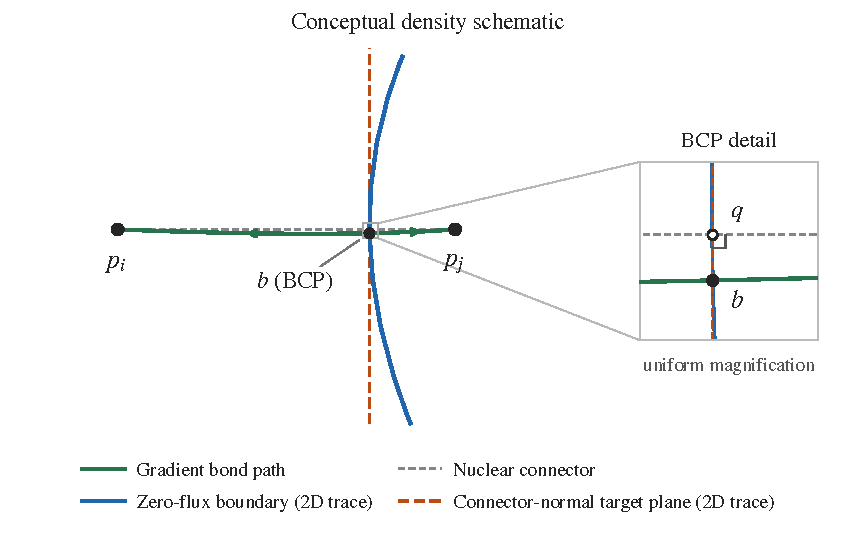
\includegraphics[width=\linewidth]{figures/figure_E_bcp_projection.pdf}
\caption{A conceptual density model in a two-dimensional section. The bond path consists of gradient-ascent branches from the BCP $b$ toward the two atomic attractors. The curved zero-flux boundary passes through $b$ and bends around the right-hand basin. The connector-normal target plane contains both $b$ and its projection $q$; the inset resolves their small separation. Passing through $b$ does not require agreement with the boundary's tangent or curvature. The geometry is illustrative, not taken from a benchmark molecule, and the plane trace does not assert a finite realized power face.}
\label{fig:bcp-projection}
\end{figure}

For fitted weights $\widehat w$, the pairwise plane $H_{ij}(\widehat w)$ has the same normal but may have a different offset. Its distance from the original BCP is exactly
\begin{equation}
 \operatorname{dist}\bigl(b,H_{ij}(\widehat w)\bigr)
 =d_{ij}\bigl|t_{ij}(\widehat w)-t_{ij}^{\mathrm{BCP}}\bigr|.
 \label{eq:bcp-plane-distance}
\end{equation}
Equation~\eqref{eq:bcp-plane-distance} explains the length error used for the fitted models. It concerns the infinite pairwise plane. Even zero distance does not place $b$ on the actual shared face: the other atoms may dominate the power distance there, as in the general distinction of Section~\ref{subsec:faces}.

Nor does a plane through one boundary point necessarily approximate the whole boundary well. Its normal is constrained by the nuclear connector, while the physical boundary can have a different tangent plane and nonzero curvature (Figure~\ref{fig:bcp-projection}). The boundary's intersection with the connector need not be $q$. A best plane approximation to a surface patch would require a choice of patch and error criterion, which is not part of these experiments. In addition, offsets from different BCPs can violate the cycle compatibility condition of Section~3. These are separate limitations of the chosen geometric family and the available observations.

\FloatBarrier
\subsection{Dataset, predictors and error aggregation}
\label{app:molecular-protocols}

The J1 benchmark contains 100 neutral singlet molecules, with 50 acyclic and 50 cyclic structures containing H, C, N, O, F, S and Cl. The dataset was assembled through deterministic PubChem searches \cite{PubChem2025}, followed by RDKit filtering and deduplication by molecular connectivity \cite{RDKit2026}. The selection records and final molecule manifest are in \path{data/qtaim_main/} of the frozen archive \cite{PowerfitArchive2026}. Its \path{scripts/qtaim/README.md} describes the calculation pipeline, and \path{results/qtaim_main/README.md} locates the J1--J4 result records.

Geometry optimization used geomeTRIC \cite{WangSong2016} with PySCF energies and gradients; the subsequent single-point calculations also used PySCF \cite{Sun2020}. Both used the B3LYP functional \cite{Becke1993,Stephens1994} and def2-SVP basis \cite{WeigendAhlrichs2005}. Multiwfn supplies the critical points and their reported atom-pair associations \cite{LuChen2012,Lu2024Multiwfn}; the reference graph uses those associations, deduplicated as unordered pairs. A separate explicit-hydrogen RDKit graph supplies the bonded label: two atoms are bonded precisely when their graph distance is one. Thus both bonded and nonbonded reference pairs can have a BCP.

The archive's reproduction environment is specified in
\texttt{environments/\allowbreak requirements-lock-py313.txt}.
It includes PySCF 2.12.1, geomeTRIC 1.1 and RDKit 2026.3.1.

J1 also records the BCP distance from the nuclear connector. A distance at most $0.02$~\AA{} occurs for 3,637 of the 3,703 bonded reference pairs ($98.22\%$), but only 3 of the 272 nonbonded pairs ($1.10\%$). This describes the landmarks' spatial distribution; by Eq.~\eqref{eq:bcp-projection}, off-axis displacement alone does not create a separator-offset error.

The proatomic inputs are spherically averaged radial electron-density profiles of isolated neutral ground-state atoms, computed with PySCF at B3LYP/def2-SVP and exported through Multiwfn. For unlike atoms separated by $d$, a bounded scalar minimization locates a minimum of
\[
 \rho_i(x)+\rho_j(d-x),\qquad 0\le x\le d.
\]
The radial profiles use piecewise cubic Hermite interpolation. Homonuclear pairs are assigned $x=d/2$. The lookup covers separations from $0.5$ to $5$~\AA{} at $0.01$~\AA{} spacing. At application time, it linearly interpolates the position $x$ and the normalized fraction $t$ separately as functions of $d$. Consequently $x_{\mathrm{lookup}}(d)$ need not equal $d\,t_{\mathrm{lookup}}(d)$ between tabulated distances. The raw proatomic length error uses the former; the fitted model takes the latter as its observations.

For an evaluated subset $S$ of pairs pooled across molecules, the reported length error is
\begin{equation}
 \operatorname{RMSE}_{\!\text{\AA}}(S)
 =\left(\frac{1}{|S|}\sum_{e\in S}\varepsilon_e^2\right)^{1/2},
 \label{eq:molecular-pooled-rmse}
\end{equation}
where $\varepsilon_e=d_e(t_e^{\mathrm{fit}}-t_e^{\mathrm{BCP}})$ for a fitted model and $\varepsilon_e=x_e^{\mathrm{lookup}}-d_e t_e^{\mathrm{BCP}}$ for the raw proatomic prediction. The midpoint error is $\varepsilon_e=d_e(1/2-t_e^{\mathrm{BCP}})$. These are not means of per-molecule RMSE; molecules with more evaluated pairs contribute more terms. J2's direct BCP-target reference fit minimizes the unweighted squared fraction errors separately on each molecule's full reference graph. In length-error notation this objective weights $\varepsilon_e^2$ by $1/d_e^2$, and it does not separately minimize the nonbonded subset error.

\subsection{Candidate graphs and realized pairs}
\label{app:molecular-candidates}

The nonperiodic molecular diagrams use atom-coordinate bounding boxes padded by $5$~\AA{} in the reference calculations. The distance cutoffs selecting J3's input pairs are a separate choice.

A realized pair is counted as \emph{visible} when the connector-line intersection belongs to its clipped face under the archived polygon-membership test \cite{Pyvoro2_063}. This numerical convention includes boundary points rather than requiring a strictly positive analytic gap. In orthonormal face coordinates measured in \AA{}, the test treats oriented edge cross products of magnitude at most $10^{-10}$~\AA$^2$ as zero. The resulting \texttt{intersection\_inside} flag supplies the visibility filter in J3 and the eligible-face selection in J4b.

Table~\ref{tab:molecular-candidates} collects the three cutoff settings. Every setting contains and realizes all 3,975 reference pairs, which are evaluated before visibility filtering. The visible subset retains 3,973 reference pairs in each setting.

\begin{table}[htbp]
\centering
\footnotesize
\setlength{\tabcolsep}{3.5pt}
\caption{J3 candidate-pair sweep. RMSE in \AA{} pools errors on all 3,975 realized reference pairs before visibility filtering. Precision and recall compare all connector-visible realized pairs, under the clipped-face convention in the text, with the fixed reference set. Counts of realized and visible pairs cover the whole diagram, including pairs outside the fitted candidates.}
\label{tab:molecular-candidates}
\begin{tabular}{@{}lrrrrrr@{}}
\toprule
\shortstack{Cutoff\\(\AA)} & Candidates & Realized & Visible & RMSE & \shortstack{Visible\\precision} & \shortstack{Visible\\recall} \\
\midrule
4.0 & 27,178 & 19,472 & 5,704 & 0.0746 & 0.6965 & 0.9995 \\
4.5 & 32,991 & 19,463 & 5,700 & 0.0770 & 0.6970 & 0.9995 \\
5.0 & 39,054 & 19,468 & 5,703 & 0.0786 & 0.6967 & 0.9995 \\
\bottomrule
\end{tabular}
\end{table}

Pairs outside the candidate set account for 2,360, 1,660 and 1,059 of the realized pairs at cutoffs $4$, $4.5$ and $5$~\AA{}, respectively; after visibility filtering, the corresponding counts are 21, 3 and 0. These counts illustrate why a score restricted to input pairs can differ from J3's whole-diagram pair evaluation. Visibility is a post hoc filter here and does not trigger a new fit.

\subsection{Local diagnostics and limits of the auxiliary checks}
\label{app:molecular-diagnostics}

J4a compares the analytic formulas with diagnostics computed from the tessellation in the reference box. The visibility decisions agree on all 38,746 recorded faces. On the 11,677 visible faces, the maximum clipped-clearance discrepancy is $3.52\times10^{-15}$~\AA{}. The population consists of faces already reported by the tessellation; this check does not test detection of missing faces.

For J4b, eligible faces are realized, connector-visible under the convention of \ref{app:molecular-candidates}, and nonbonded under the RDKit convention. Faces from all molecules are pooled separately for the ordinary Voronoi model and the J3 power fit at the $5$~\AA{} cutoff. The ranked clearance is $c_{ij}^{\Omega}$ from Eq.~\eqref{eq:clipped-clearance}; both clearance and face area refer to the clipped reference-box diagrams. Each population is ranked by decreasing clearance, decreasing face area, or increasing pair distance. Writing $y_k\in\{0,1\}$ for the QTAIM-reference label at rank $k$ and $N_+=\sum_k y_k$, the archived average precision is
\[
 \operatorname{AP}
 =\frac{1}{N_+}\sum_k y_k\,
   \frac{\sum_{\ell\le k}y_\ell}{k}.
\]
It is the mean precision at the ranks occupied by positive reference pairs. The archived stable sort preserves record order for equal scores. This calculation is performed once on each pooled population, rather than averaging molecule-level AP values. The exploratory clearance cutoff of $0.50$~\AA{} in the source archive is not a calibrated classification rule.

The additional J4c molecular illustrations use fits to projected BCP targets, not J3's proatomic candidate observations. They are therefore not used here as evidence for that prediction pipeline. J4d varies box margins over $3$, $5$, $7$ and $10$~\AA{}. Voronoi geometries are recomputed, giving 18,798, 19,278, 19,605 and 19,830 realized-pair records. In contrast, all 19,468 recovered-powerfit records are reused unchanged at each margin. These repetitions do not independently establish robustness of the recovered-powerfit geometry to a changed clipping box.

% Sources: frozen powerfit-80933a1 archive, data/qtaim_main and results/qtaim_main.
% BCP associations: scripts/qtaim/run_multiwfn_topology.py, parse_multiwfn_output.
% Proatomic predictor: scripts/qtaim/_proatomic_pairlaw.py and data/proatomic/.
% J2/J3 pooling: analyze_qtaim_true_support_ladder.py / analyze_qtaim_candidate_recovery.py.
% AP definition: scripts/build_manuscript_tables.py, _average_precision and
% table_j4_clearance_ranking; the tie convention is retained from that source.
% Figure E is a deliberately chosen geometric schematic, not molecular data.
